\documentclass{beamer}
%\usepackage[utf8]{inputenc}
%\usetheme{Frankfurt}  %% Themenwahl
\beamertemplatenavigationsymbolsempty


\setbeamertemplate{footline}[frame number]
%\setbeamertemplate{bibliography item}{[\theenumiv]}
%\input{paper-layout}
%\usepackage{ngerman}
\usepackage{hyperref}
\usepackage[latin1]{inputenc}
\usepackage{amssymb}
\usepackage{amsmath}
%\input{german}

%\usepackage{cite} 
\usepackage{tikz}
\usetikzlibrary{automata,positioning}
\usepackage{cleveref}
%\usepackage{algorithm}
%\usepackage[noend]{algpseudocode}
%\usepackage{algorithmic}


%%
\PassOptionsToPackage{table,svgnames,dvipsnames}{xcolor}

%\usepackage[utf8]{inputenc}
\usepackage[T1]{fontenc}
\usepackage[sc]{mathpazo}



\usepackage[ngerman,american]{babel}
\usepackage[autostyle]{csquotes}
\usepackage[%
backend=biber,
url=false,
style=ieee,
maxnames=4,
minnames=3,
maxbibnames=99,
giveninits,
uniquename=init]{biblatex} % TODO: adapt citation style
\usepackage{graphicx}
\usepackage{scrhack} % necessary for listings package
\usepackage{listings}
\usepackage{lstautogobble}
\usepackage{tikz}
\usepackage{float}

\usepackage{ifluatex}
\ifluatex
\usepackage{pdftexcmds}
\makeatletter
\let\pdfstrcmp\pdf@strcmp
\let\pdffilemoddate\pdf@filemoddate
\makeatother
\fi
\usepackage{svg}

\usetikzlibrary{calc, positioning, fit, shapes.misc}
\tikzstyle{vertex} = [fill,shape=circle,node distance=80pt]
\tikzstyle{edge} = [fill,opacity=.5,fill opacity=.5,line cap=round, line join=round, line width=50pt]
\tikzstyle{elabel} =  [fill,shape=circle,node distance=30pt]
\pgfdeclarelayer{background}
\pgfsetlayers{background,main}

\usepackage{pgfplots}
\usepackage{pgfplotstable}
\usepackage{booktabs}
\usepackage[final]{microtype}
\usepackage{caption}
%\usepackage[hidelinks]{hyperref} % hidelinks removes colored boxes around references and links

\bibliography{bibliography}

%\setkomafont{disposition}{\normalfont\bfseries} % use serif font for headings
\linespread{1.05} % adjust line spread for mathpazo font

% Add table of contents to PDF bookmarks
\BeforeTOCHead[toc]{{\cleardoublepage\pdfbookmark[0]{\contentsname}{toc}}}

% Define TUM corporate design colors
% Taken from http://portal.mytum.de/corporatedesign/index_print/vorlagen/index_farben
\definecolor{TUMBlue}{HTML}{0065BD}
\definecolor{TUMSecondaryBlue}{HTML}{005293}
\definecolor{TUMSecondaryBlue2}{HTML}{003359}
\definecolor{TUMBlack}{HTML}{000000}
\definecolor{TUMWhite}{HTML}{FFFFFF}
\definecolor{TUMDarkGray}{HTML}{333333}
\definecolor{TUMGray}{HTML}{808080}
\definecolor{TUMLightGray}{HTML}{CCCCC6}
\definecolor{TUMAccentGray}{HTML}{DAD7CB}
\definecolor{TUMAccentOrange}{HTML}{E37222}
\definecolor{TUMAccentGreen}{HTML}{A2AD00}
\definecolor{TUMAccentLightBlue}{HTML}{98C6EA}
\definecolor{TUMAccentBlue}{HTML}{64A0C8}

% Settings for pgfplots
\pgfplotsset{compat=newest}
\pgfplotsset{
	% For available color names, see http://www.latextemplates.com/svgnames-colors
	cycle list={TUMBlue\\TUMAccentOrange\\TUMAccentGreen\\TUMSecondaryBlue2\\TUMDarkGray\\},
}

% Settings for lstlistings
\lstset{%
	basicstyle=\ttfamily,
	columns=fullflexible,
	autogobble,
	keywordstyle=\bfseries\color{TUMBlue},
	stringstyle=\color{TUMAccentGreen}
}


\usepackage{amssymb}
\usepackage{amsmath}
\usepackage{algorithm}
\usepackage[noend]{algpseudocode}
\usepackage{cleveref}
%\newtheorem{theorem}{Theorem}%[section] 
%\usepackage{algorithm2e}
\newtheorem{sdp}{SDP}
\usepackage[long]{optidef}

\usepackage{pifont}% http://ctan.org/pkg/pifont
\newcommand{\cmark}{\ding{51}}%
\newcommand{\xmark}{\ding{55}}

\usepackage{varwidth}

%%

\title{Spectral Methods to Find Small Expansion	Sets on Hypergraphs}

\author{Bachelor's Thesis in Informatics}
\institute{	Franz Rieger\\Department of Informatics\\Technical University of Munich\\
	Supervisor: Prof. Dr. rer. nat. Susanne  Albers\\
	Advisor: Dr. T.-H. Hubert Chan\\
	Submission Date: 15. March 2019\\
	%Presentation Date: 19. March 2019
	%\href{mailto:franz.rieger@cs.tum.edu}{franz.rieger@cs.tum.edu} 
}
	

\date{19. March 2019}

\begin{document}
	\maketitle
%	\frame{\tableofcontents[currentsection]}
	
	\section{Motivation}
	\begin{frame} %%Eine Folie
		\frametitle{Motivation} %%Folientitel
			\begin{itemize}
				\item graph theory interest
				\item find group of friends in social networks
				\item heuristics for combination games
			\end{itemize}
			
		$\to$ small expansion sets
	\end{frame}
	
	\section{Hypergraphs}
	\begin{frame}
		\frametitle{Hypergraphs}
		
		\begin{itemize}
			\item
			weighted, undirected (hyper)graph $H = (V, E, w)$
			\item  $n$ vertices $V = \{v_1, \ldots, v_n\}$ 
			\item
		 $m$ (hyper-)edges $E = \{ e_1, \ldots , e_m | \forall i \in [i]: e_i \subseteq V \land e_i \neq \emptyset \} $ every edge $e$ is non-empty subset of $V$ 
		 \item  positive edge weights $w_e:= w(e) $; weight function $w: E \to  \mathbb{R}_+ $
			
			\begin{tikzpicture}
			\node[vertex,label=below:\(v_1\)] (v1) {};
			\node[vertex,right of=v1,label=below:\(v_2\)] (v2) {};
			\node[vertex,right of=v2,label=below:\(v_3\)] (v3) {};
			\node[vertex,below of=v2,label=below:\(v_4\)] (v4) {};	
			
			\begin{pgfonlayer}{background}
			\draw[edge,color=yellow] (v1) -- (v2) -- (v3);
			
			\begin{scope}[transparency group,opacity=.5]
			\draw[edge,opacity=1,color=blue,line width=40pt] (v2) -- (v3) -- (v4) --(v2);
			\fill[edge,opacity=1,color=blue] (v2.center) -- (v3.center) -- (v4.center) -- (v2.center);
			
			\end{scope}
			
			
			\end{pgfonlayer}
			
			\node[elabel,color=yellow,label=right: {$e_1 , w_{e_1} = 0.7$}]  (e1) at (-4,0) {};
			
			\node[elabel,below of=e1,color=blue,label=right:{$e_2, w_{e_2} = 1.3$}]  (e2) {};
			
			\end{tikzpicture}
		An example for a simple hypergraph with four vertices and two hyperedges. $G=(\{v_1, v_2, v_3, v_4\},\{\{v_1, v_2, v_3\}, \{v_2,v_3, v_4\}\} )$\label{fig:exapmlehypergraph}	
		\end{itemize}
	\end{frame}
	\begin{frame}
	\frametitle{Hypergraphs}
		
		
	\begin{itemize}
	\item degree of a vertex $v\in V$:  $deg(v) := |\{e\in E: v\in e\}|$
	\item   $\forall v\in V : deg(v) =d $: hypergraph $d$-regular
		\item  $\forall e\in E : |e| =r $ : hypergraph $r$-uniform

	
	\end{itemize}
		
	
		
	

	\end{frame}
	\section{Edge expansion}
	\begin{frame}
		\frametitle{Edge expansion}
		\begin{itemize}
			
			\item 
			 set of edges which are cut by  $S$ : $
			\partial S:= \{e\in E : e \cap S \neq \emptyset \land  e \cap (V \setminus S) \neq \emptyset  \}
			$
			\item weight $w_v$ of a vertex $v$: $
			w_v := \sum_{e\in E: v\in e} w_e
		$ %Accordingly, a subset $S\subseteq V$ of vertices has weight $w_S := \sum_{v\in S} w_v$ and a subset $F \subseteq E $ of edges has weight $w_F = \sum_{e\in F} w_e$.
			\item  weight $w(S)$ of a set $S$ of vertices : 
			$
			w(S) := \sum_{v\in S} w_v
			$
			\item weight $w(F)$ of a set $F$ of edges : 
		$
			w(F) := \sum_{e\in F} w_e
		$
			\item
			 edge expansion of a set of vertices $\emptyset \neq S \subseteq V$ : \begin{equation}
			\Phi(S):= \frac{w(\partial S)}{w(S)}
			\end{equation}
			\item  expansion of a graph $H$: \begin{equation}
			\Phi(H) := \min_{\emptyset \subsetneq S \subsetneq V} \max \{\Phi(S), \Phi(V\setminus S)\}
			\end{equation} 
		\end{itemize}
	\end{frame}

\begin{frame}	
\frametitle{Edge expansion}
		
			\begin{itemize}
				\item 		non-connected graphs: $\Phi(H) = 0$ 
					\begin{figure} [htpb]
					\centering
					\begin{tikzpicture}[scale = 0.1]
					\node[vertex,label=below:\(v_1\)] (v1) {};
					\node[vertex,right of=v1,label=below:\(v_2\)] (v2) {};
					\node[vertex,right of=v2,label=below:\(v_3\)] (v3) {};
					\node[vertex,below of=v2,label=below:\(v_4\)] (v4) {};	
					\node[vertex,below of=v3,label=below:\(v_5\)] (v5) {};	
					\node[vertex,right of=v5,label=below:\(v_6\)] (v6) {};	
					\begin{pgfonlayer}{background}
					\draw[edge,color=yellow] (v1) -- (v2) -- (v3);
					\draw[edge,color=green] (v5) -- (v6) ;
					
					\begin{scope}[transparency group,opacity=.5]
					\draw[edge,opacity=1,color=blue,line width=40pt] (v2) -- (v3) -- (v4) --(v2);
					\fill[edge,opacity=1,color=blue] (v2.center) -- (v3.center) -- (v4.center) -- (v2.center);
					
					\end{scope}
					
					
					\end{pgfonlayer}
					
					\node[elabel,color=yellow,label=right: {$e_1 , w_{e_1} = 0.7$}]  (e1) at (-4,-14) {};
					
					\node[elabel,below of=e1,color=blue,label=right:{$e_2, w_{e_2} = 1.3$}]  (e2) {};
					\node[elabel,below of=e2,color=green,label=right:{$e_3, w_{e_3} = 1.5$}]  (e3) {};
					
					\end{tikzpicture}
					\caption[Example non-connected hypergraph]{An example for a non-connected hypergraph with two connection components. For $S:= \{v_5, v_6\} $ it can be verified that $\delta S = \emptyset$, hence $\Phi(S) =\Phi(V\setminus S) = 0$. }\label{fig:exapmle_non_connected_hypergraph}
				\end{figure}
			\item 
			 expansion $\Phi(H)$ is NP-hard \cite{kaibel2004expansion}
			
			\end{itemize}

		
		
			
		
	
			
			
			
			
			
	
		

\end{frame}
	
	

	\begin{frame}
	\frametitle{Discrepancy ratio}
\begin{itemize}
			\item 
			 discrepancy ratio, given a non-zero vector $f \in \mathbb{R}^V$: \begin{equation}\label{eq:discrepancy_ratio}
			D_w(f) := \frac{\sum_{e\in E} w_e \max_{u,v\in e}(f_u - f_v)^2}{\sum_{u\in V} w_u f_u^2}
			\end{equation} 

			\item  connected to the edge expansion $\Phi(S)$ of a set $S$ if   $f$ is indicator vector for $S$
			\begin{itemize}
					\item  nominator $\sum_{e\in E} w_e \max_{u,v\in e}(f_u - f_v)^2$ would sum over all the edges in $\delta S$
				\item   denominator $\sum_{u\in V} w_u f_u^2$  would sum over the vertices $S$
				\item $	D_w(f) = \frac{w(\delta S)}{w(S)} = \Phi(S)$
			\end{itemize}
			
		
			
			
			
			%The discrepancy ratio can also be defined on the so called normalized space with $x\in \mathbb{R}^V$:
			%\begin{equation}
			%\mathcal{D}(x) = D_w(W^{-\frac{1}{2}}x)
			%\end{equation}
			\item  orthogonal minimaximizer :  lowest discrepancy value of $k$ mutually orthogonal non-zero vectors:
			\begin{equation}\label{eq:xi}
			\xi_k := \min_{0 \neq f_1, \ldots , f_k ; f_i \perp f_j } \max_{i \in [k]} D_w(f_i)
			\end{equation}

			
		
		\end{itemize}
			
		\end{frame}

	\section{Algorithms}



\begin{frame}
	\frametitle{Approximation of small expansion sets}

		\begin{theorem}{(Theorem 8.1 in \cite{ChanLTZ16}) \label{theorem:small_discrepancy_ratio}}
		There exists a randomized polynomial time algorithm that, given a hypergraph $H = (V,E,w)$ and a parameter $ k < |V |$, outputs $k$ orthonormal vectors $f_1, \ldots , f_k$ in the weighted space such that with high probability, for each $i  \in [k],$
		\begin{equation}
		D_w(f_i) \le \mathcal{O} (i \xi_i \log r  ) 
		\end{equation}	
	\end{theorem}
\end{frame}


\begin{frame}
	\begin{theorem}{(Theorem 6.6 in \cite{ChanLTZ16})}\label{theorem:small_xi}
		Given a hypergraph $H = (V, E, w)$ and $k$ vectors $f_1, f_2, \ldots , f_k$ which are orthonormal in the weighted space with $ \max_{s \in [k]} D_w(f_s) \le \xi $, the following holds: Algorithm \ref{alg:small_set_expansion} constructs a random set $S \subsetneq V$ in polynomial time such that with $\Omega(1)$ probability, $|S| \le \frac{24|V|}{k}$ and
		\begin{equation}\label{eq:small_expansion}
		\phi(S) \le C \min\{\sqrt{r \log k}, k \log k  \log \log k \sqrt{\log r} \} \cdot \sqrt{\xi},
		\end{equation}
		where $C$ is an absolute constant and $r := \max_{e\in E} |e|$.
	\end{theorem}
\end{frame}


\begin{frame}
	Deducted from \cite{ChanLTZ16}
\begin{algorithm}[H]
	\caption{Find Small Expansion Set \label{alg:ses}} 
	\begin{algorithmic}[0]
		\Function{SmallExpansionSet}{$H, k$}
		\State $f_1 \ldots, f_k := $\Call{SampleSmallVectors}{$H, k$}
		\State return \Call{SmallSetExpansion}{$H, f_1 \ldots, f_k$}
		\EndFunction 
	\end{algorithmic}
\end{algorithm}	
\end{frame}


\begin{frame}

\frametitle{Brute-force graph expansion}
\begin{algorithm}[H]
	\caption{Brute-force edge expansion on a hypergraph \label{alg:brute_force}}
	\begin{algorithmic}[0]
		\Function{BruteForceEdgeExpansion}{$H := (V,E, w)$}
		\State $bestS := null$
		\State $lowestExpansion := \infty$
		\For{$\emptyset \neq S \subsetneq V$}
		\State $expansion :=  \max\{ \Phi(S), \Phi({V\setminus S})\}$
		\If{$expansion < lowestExpansion$}
		\State $lowestExpansion := expansion$
		\State $bestS := S$
		\EndIf
		\EndFor	
		\State return $bestS$
		\EndFunction
	\end{algorithmic}
\end{algorithm}
Runtime complexity:  $2^{|V|}-2 = 2^{n}-2 \in O(2^n) $ combinations for $\emptyset \neq S \subsetneq V$
\end{frame}


\begin{frame}

\frametitle{Brute-force set expansions}
\begin{algorithm}[H]
\caption{Brute-force expansion of sets for every size   \label{alg:brute_force_size_just_one_side}}
\begin{algorithmic}[0]
	\Function{BruteForceEdgeExpansionSizesSets}{$H := (V,E, w)$}
	\State $bestSofSize := \{\}$
	\State $lowestExpansionOfSize := \{1:\infty, 2:\infty, \ldots, n-1: \infty \}$
	\For{$\emptyset \neq S \subsetneq V$}
	\State $expansion :=  \Phi(S)$
	\If{$expansion < lowestExpansionOfSize[|S|]$}
	\State $ lowestExpansionOfSize[|S|] := expansion$
	\State $bestSofSize[|S|] := S$
	\EndIf
	\EndFor	
	\State return $bestSofSize$
	\EndFunction
\end{algorithmic}
\end{algorithm}

\end{frame}

\section{Random Hypergraphs}
\begin{frame}
\frametitle{Random Hypergraphs}
	\begin{itemize}
		\item r-uniform
		\item d-regular
		\item unique edges guaranteed
		\item connected guaranteed
		\item guaranteed to terminate
		\item polynomial time complexity
		\item all possible graphs
		\item all with equal probability
	\end{itemize}

\end{frame}
\begin{frame}


\frametitle{Adding random edges}

\begin{algorithm}[H]
	\caption{Generate by adding random edges\label{alg:simple_random_graph}} 
	\small
	\begin{algorithmic}
		\Function{GenerateAddRandomEdges}{$n, r, numberEdges, weightDistribution$}
		\State $E := \emptyset$
		\State $V := \{v_1, \ldots, v_n\}$
		\State $w = \{\}$
		\For{$1, \ldots , numberEdges$}
		\State $nextEdge := sample(V, r) $
		\State $E := E \cup	 \{nextEdge\}$ % \Comment only sample edges which do not already exist
		\State $weight(nextEdge) := sample(weightDistribution)$ 
		\EndFor
		\State return $H = (V, E, w)$
		\EndFunction 
	\end{algorithmic}
\end{algorithm}	
$numberEdges = \lceil\frac{nd}{r}\rceil$ according to \cref{eq:ndmr}
\end{frame}
\begin{frame}


\begin{algorithm}[H]
	\caption{Generate random graph with resampling\label{alg:GenerateRandomGraphWithResampling}} 
	\small
	\begin{algorithmic}
		\Function{GenerateRandomGraph}{$n, r, d, weightDistribution$}
		\State $G:=$ \Call{GenerateAddRandomEdges}{$n, r, \frac{nd}{r}, weightDistribution$}
		\While{$\text{not connected}(G)$ }%or $ \exists e,f \in E. e = f$}
		\State $G:=$ \Call{GenerateAddRandomEdges}{$n, r, \frac{nd}{r}, weightDistribution$}
		\EndWhile
		\State return $G:=(V,E)$	
		\EndFunction 
	\end{algorithmic}
\end{algorithm}	
\end{frame}


\begin{frame}
\begin{algorithm}[H]%[htpb]
	\caption{Generate random graph by creating a spanning tree\label{alg:spanning_tree}} 
	\tiny
	\begin{algorithmic}[0]
		\Function{GenerateWithSpanningTree}{$n, r, d, weightDistribution$}
		\State $V := \{v_1, \ldots, v_n\}$
		\State $w = \{\}$
		\State $firstEdge := choice(V,r)$
		\State $w(firstEdge) = sample(weightDistribution) $
		\State $E := \{firstEdge\}$
		\While {$\{v\in V| deg(v) = 0 \} \neq \emptyset$} \Comment create tree
		\If{ $|\{v\in V| deg(v) = 0 \}| \ge r-1$}
		\State $nextEdgeTreeVertex := choice(\{v\in V| deg(v) = 1 \})$\Comment get one tree node
		\State\begin{varwidth}[t]{\linewidth}
			$nextEdgeVertices :=$ \par
			\hskip\algorithmicindent $ choice(\{v\in V| deg(v) =0\}, r-1) \cup \{nextEdgeTreeVertex\}$\par
		\end{varwidth}
		\Else
		\State \begin{varwidth}[t]{\linewidth}
			$nextEdgeVertices :=  \{v\in V| deg(v) =0\}  \cup$ \par
			\hskip\algorithmicindent $  choice(\{v\in V| deg(v) =1\}, r-| \{v\in V| deg(v) =0\}| )$\par
		\end{varwidth}
		\EndIf
		\State $nextEdge := nextEdgeVertices$
		\State $E := E \cup \{nextEdge\}$
		\State $w(nextEdge):=  sample(weightDistribution)$
		\EndWhile
		\While{$|\{v\in V| deg(v)< d\}| \ge r$} \Comment fill up degrees
		\State $ smallestDegreeVertices := \{v\in V| deg(v) = \min_{u\in V} deg(u) \}$
		\If {$|smallestDegreeVertices| >= r$}
		\State $nextEdgeVertices := sample(smallestDegreeVertices, r) $ \State \Comment draw without replacement
		\Else
		\State $secondSmallestDegreeVertices := \{v\in V| deg(v) = \min_{u\in V} deg(u) +1 \}$
		\State \begin{varwidth}[t]{\linewidth}
			$nextEdgeVertices :=$ \par
			\hskip\algorithmicindent $ sample(secondSmallestDegreeVertices, r - | smallestDegreeVertices|)$\par
		\end{varwidth}
		\State $nextEdgeVertices := smallestDegreeVertices \cup nextEdgeVertices  $
		\EndIf
		
		\State $nextEdge := nextEdgeVertices$
		\State $E := E \cup \{nextEdge\}$
		\State $w(nextEdge):= sample(weightDistribution)$
		\EndWhile
		\State return $G:=(V,E, w)$	
		\EndFunction 
	\end{algorithmic}
\end{algorithm}	
\end{frame}

\begin{frame}
\frametitle{Implementation}
\begin{itemize}
	\item focus on demonstrating feasibility, not runtime performance
	\item Python + NumPy + SciPy
	\item own implementation of hypergraphs, vertices and edges
	\item \href{https://github.com/riegerfr/Bachelor-s-thesis-edge-expansion/tree/master/hypergraph-implementation}{https://github.com/riegerfr/Bachelor-s-thesis-edge-expansion/tree/master/hypergraph-implementation}
\end{itemize}



\end{frame}

\section{Evaluation}
\begin{frame}
\frametitle{Runtime input graph sizes}
\begin{figure}[H]
	\centering
	\includegraphics[scale=0.5]{figures/number_vertices_all_logs.pdf}
	\caption[Plot graph size against time]{Plot of the number of vertices $n$ in the graphs against the time for computing solutions. It can be seen that the brute-force algorithm takes a long time for larger graphs, while the approximation algorithm's time only increases slowly.\label{fig:no_vertices_time}}
\end{figure}
\end{frame}


\begin{frame}
\frametitle{Runtime for different k}
	\begin{figure}
		\centering
		\includegraphics[scale=0.5]{figures/k_all_logs.pdf}
		\caption[Plot k against time]{Plot of $k$ against the runtime for the approximation algorithm with the constant brute-force time for comparison. For higher k outliers occur.\label{fig:k_time}}
	\end{figure}
\end{frame}

\begin{frame}
\frametitle{Small expansion sizes}
\begin{figure}
	\centering
	\includegraphics[scale=0.5]{figures/quality_evaluation_log_small_expansion_sizes.pdf}
	\caption[Plot sizes small expansions]{Plot of sizes of the expansions generated by the approximation algorithm.\label{fig:sizes_small_expansions}}
\end{figure}
\end{frame}

\begin{frame}
\frametitle{Random graphs expansion comparison}
\begin{figure}
	\centering
	\includegraphics[scale=0.5]{figures/creation_algorithm_log_lowest_expansion.pdf}
	\caption[Plot lowest expansion for different algorithms]{Plot of the lowest expansion values of graphs created by different algorithms for each size of the expansion set. \label{fig:plot_lowest_expansion_each_size}}
\end{figure}

\end{frame}

\begin{frame}
\frametitle{Estimation of C}
	\begin{equation} \label{eq:c_estimate}
	C\ge \frac {\phi(S)}{ \min\{\sqrt{r \log k}, k \log k  \log \log k \sqrt{\log r} \} \cdot \sqrt{\xi}}
	\end{equation}
	
	\begin{figure}
		\centering
		\includegraphics[scale=0.4]{figures/quality_evaluation_log_C_estimates.pdf}
		\caption[Plot C estimates]{Plot of estimates for the constant C in \cref{theorem:small_xi} for $k=3$. Interestingly, $\max C \approx 2.71 \approx e$\label{fig:c_estimates} }
	\end{figure}
	
\end{frame}
\begin{frame}
\frametitle{Expansion comparison estimate/brute-force}
\begin{figure}
	\centering
	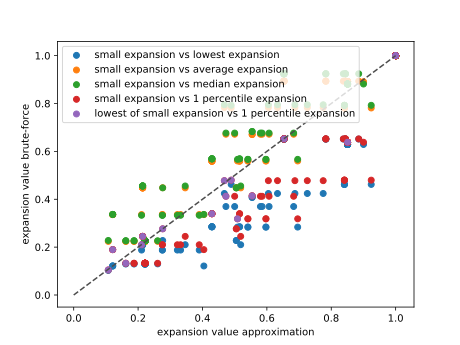
\includegraphics[scale=0.5]{figures/quality_evaluation_log_expansion_values_for_same_number_verticies.pdf}
	\caption[Plot expansions approximation against brute force]{\footnotesize Plot of the expansion values achieved by the small expansion set approximation algorithm against the expansion set of the same size with the lowest expansion (as generated through the brute-force approach). Entries below the diagonal line signal that the expansion found by the approximation algorithm was worse than the set found by the brute force algorithm. \label{fig:expansion_approx_vs_brute}}
\end{figure}
\end{frame}

\section{Applications}
\begin{frame}
\frametitle{Applications}
	\begin{itemize}
		\item Hypergraph representation of social networks: users as vertices, interactions as edges
		\item Small expansion approximation: group of friends
		\item Other application: small expansion set as heuristics in combination games
	\end{itemize}
\end{frame}
	
		
	\section{Wrap up}
	\begin{frame}
		Wrap up:
		
		\begin{itemize}
		
			\item edge expansion NP-hard
			\item approximation algorithm for small expansion set
			\item random hypergraphs
			\item find group of friends in social networks
			
		\end{itemize}
	\end{frame}
	
	\begin{frame}
			Thank you! 
			Questions?
	\end{frame}


%\bibliographystyle{IEEEtran}
% argument is your BibTeX string definitions and bibliography database(s)
%\nocite{*}
\begin{frame}[allowframebreaks]
	\frametitle{References}
\printbibliography{}
\end{frame}


		\begin{frame}
		\frametitle{Backup slides}
		\end{frame}
		
	
	\begin{frame}
	\frametitle{Creation of orthogonal vectors with low discrepancy ratio}
	

	
	\begin{algorithm}[H]
		\caption{Procedural Minimizer \label{alg:procedural_minimizer}} 
		\begin{algorithmic}
			\Function{SampleSmallVectors}{$H,k$}
			\State $f_1= \frac{\vec{1}}{||\vec{1}||_w}$
			
			\For{$i = 2, \ldots, k$}
			\State $f_i := $\Call{SampleRandomVector}{$H, f_1, \ldots, f_{i-1}$}
			\State $f_i = \frac{f_i}{||f_i||_w}$
			\EndFor
			\State return $f_1, \ldots , f_k$
			\EndFunction 
		\end{algorithmic}
	\end{algorithm}	
	
\end{frame}
\begin{frame}

\begin{sdp}{Semidefinite programming problem for minimizing $g$ (SDP 8.3 in \cite{ChanLTZ16}) \label{SDP}} %todo: better name, where from
\begin{mini*}
	{g}{\text{SDPval} := \sum_{e\in E} w_e \max_{u,v\in e} ||\vec{g_u} -\vec{g_v} ||^2}{}{}
	\addConstraint{ \sum_{u\in V} w_v ||\vec{g_v}||^2 }{= 1}{}
	\addConstraint{ \sum_{u\in V} w_v f_i(v)  \vec{g_v} }{=\vec{0},\quad}{\forall i \in [k-1]}
\end{mini*}


\begin{algorithm}[H]
	\caption{Sample Random Vector (Algorithm 3 in \cite{ChanLTZ16}) \label{alg:sample_random_vector}} 
	\begin{algorithmic}
		\Function{SampleRandomVector}{$H, f_1, \ldots, f_{i-k}$}
		\State Solve SDP \ref{SDP} to generate vectors $\vec{g_v} \in \mathbb{R}^n $ for $v \in V$
		\State $\vec{z} := sample(\mathcal{N}(0,I_n))$\Comment random gaussian vector
		\For{$v\in V $}
		\State $f(v) := \langle \vec{g_v}, \vec{z} \rangle$
		\EndFor
		\State return $f$
		\EndFunction 
	\end{algorithmic}
\end{algorithm}	

\end{sdp}
\end{frame}

\begin{frame}
\frametitle{Calculating a small expansion set}

\end{frame}
\begin{frame}

\begin{algorithm}[H]
\caption{Small Set Expansion (according to Algorithm 1 in \cite{ChanLTZ16}) \label{alg:small_set_expansion}} %todo: better name


\begin{algorithmic}
\Function{SmallSetExpansion}{$G := (V,E, w), f_1, \ldots , f_k$}
%	\State assert $\xi == \max_{s\in [k]} \{D_w(f_s)\}$
%	\State assert $\forall f_i, f_j \in \{f_1, \ldots , f_k\} \subset \mathbb{R}^n, i\neq j: f_i \text{ and } f_j \text{ orthonormal in weighted space} $

\For{$v \in V, s\in [k]$}
\State	$u_v(s) := f_s(v) $
\EndFor


\For{$v \in V$}
\State $\tilde{u}_v := \frac{u_v}{||u_v||}$
\EndFor

\State $\hat{S} := $ \Call{OrthogonalSeparator}{$\{\tilde{u}_v\}_{v\in V} , \beta = \frac{99}{100}, \tau = k$ }

\For {$v \in V$}
\If {$\tilde{u}_v \in \hat{S}$ }

\State $X_v := ||u_v||^2$
\Else
\State $X_v := 0$
\EndIf

\EndFor
\State $X:= $ sort $ list(\{X_v\}_{v \in V})$
\State $V := [v]_{\text{in order of X}}$
\State $S := \arg \min_{\{P \text{ is prefix of }V\}}\phi(P)$

\State return $S$



\EndFunction


\end{algorithmic}
\end{algorithm} %todo: explain list syntax in notation
\end{frame}

\begin{frame}
\begin{algorithm}[H]
\caption{Orthogonal Separator (combination of Lemma 18 and algorithm of Theorem 10 in \cite{LouisM14}; also Fact 6.7 in \cite{ChanLTZ16}) \label{alg:orthogonal_separator}} 

\begin{algorithmic}
\Function{OrthogonalSeparator}{$\{\tilde{u}_v\}_{v\in V} , \beta = \frac{99}{100}, \tau = k$}
\State $l := \lceil \frac{\log_2 k}{1-\log_2 (1+\frac{2}{log_2 k})}\rceil$



\State $w := $\Call{SampleAssignments}{$\{\tilde{u}_v\}_{v\in V},l, V, \beta$}

\For{$ v \in V$}
\State $W(v) := w_1(v)w_2(v)\cdots w_l(v)$
\EndFor

\If{$n\ge 2^l$}
\State $word := random( \{0,1\}^l)$ \Comment uniform

\Else

\State $words := set({W(v): v\in V})$ \Comment no multiset
\State $words = words \uplus \{w_1, \ldots , w_{|V|-|words|} \in \{0,1\}^l\} $ 
\State $word := random(words)$ \Comment uniform

\EndIf

\State $r := uniform(0,1)$
\State $S := \{v \in V: ||\tilde{u}_v||^2 \ge r \land W(u) = word \}$
\State return $S$

\EndFunction %todo: 1-vector explain;
%todo: explain norm
%todo: i or u or v for what?
\end{algorithmic}
\end{algorithm}	
\end{frame}
\begin{frame}
\begin{algorithm}[H]
\caption{Sample Assignments (proof of Lemma 18 in \cite{LouisM14}) \label{alg:sample_assignments}} 
\begin{algorithmic}
\Function{SampleAssignments}{$\{\tilde{u}_v\}_{v\in V},l, V, \beta$}
\State $\lambda := \frac{1}{\sqrt{\beta}}$
\State $k:= |\tilde{u}|$ \Comment number of entries for each vertex
\State $g:=$ sample($\mathcal{N}(0,I_k)$) \Comment all components $g_i$ mutually indep.

\State $poisson\_process := N(\lambda)$ \Comment Poisson process on $\mathbb{R}$ w. rate $\lambda$

\For {$i = 1, 2, \ldots, l$}
\For{$v\in V$}


\State $t := \langle g, \tilde{u}_v \rangle $
\State $poisson\_count := poisson\_process(t)$ 
\State\Comment \# events between $t=0$ and $t_v$
\If{$poisson\_count \mod 2 == 0 $}
\State $w_i(v) := 1$
\Else
\State  $w_i(v) := 0$
\EndIf
\EndFor
\EndFor
\State return $w$
\EndFunction %todo: 1-vector explain
\end{algorithmic}
\end{algorithm}	


\end{frame}
	
	\begin{frame}
	
	\frametitle{Notation}
	\begin{itemize}
		
		
		
		%The notation used in this thesis is orientated on \cite{ChanLTZ16}.
		
		%In the algorithms, values are assigned to each vertex $v\in V$ in the form of vectors $f, g \in \mathbb{R}^V$. %These values can be defined in the so-called weighted space but also transformed to the normalized space, which are equivalent up to a transformation. Vectors in the weighted space are commonly denoted by $f,g\in \mathbb{R}^V$ and are related to vectors in the normalized space $x,y \in \mathbb{R}^V$ by $x = W^\frac{1}{2}f$. 
		\item  vectors $f, g \in \mathbb{R}^V$ the inner product is defined as $ \langle f,g \rangle_w := f^T W g$.
		\item 	If $ \langle f,g \rangle_w   = 0 $, $f$ and $g$ are said to be orthogonal
		\item  norm  $||f||_w := \sqrt{ \langle f,f \rangle_w}$
		\item  weight matrix $W$ of a hypergraph \begin{equation}
		W := 
		\begin{pmatrix}
		w_{v_1} & 0 & 0&\dots &0 \\
		0 & w_{v_2} & 0 & \ldots & 0 \\
		0 & 0 & w_{v_3} & \ldots & 0 \\
		\vdots & \vdots & \vdots & \ddots & \vdots \\
		0 &0&0& \ldots  & w_{v_n}
		\end{pmatrix} \in \mathbb{R}_{0+}^{n \times n} 
		\end{equation} 
	\end{itemize}
\end{frame}
\begin{frame}\begin{itemize}
							\item  $0\le D_w(f) \le 2 $ \cite{ChanLTZ16}
							\item $0\le \Phi(H)\le 1$ 
							
							
							
							\item  $d$-regular, $r$-uniform hypergraphs (handshaking theorem):
							\begin{equation}\label{eq:ndmr}
							n d = m r
							\end{equation}
							
							
							
							\item  path between two vertices $v_1,v_k\in V$ : list of vertices $v_1, v_2 \ldots , v_k$ where each tuple of vertices following another is connected by an edge, i.e. $\forall i \in [k-1]\exists e \in E: u_i, u_{i+1} \in e  $
							\item  connected component :  $S\subseteq V. \forall u,v \in S . \exists path(u,v)$
							\item  $S=V$: hypergraph connected
\end{itemize}

\end{frame}


\begin{frame}
\frametitle{Runtime rank/degree-combinations}
\begin{figure}[H]
	\centering
	\includegraphics[scale=0.5]{figures/rank_degree_combinations_all_logs.pdf}
	\caption[Plot rank degree combinations against time]{Plot of runtimes for different (rank, degree) combinations.\label{fig:rank_degree_times}}
\end{figure}
\end{frame}



\begin{frame}
\begin{algorithm}[H]
	\caption{Generate random hypergraph, sampling from lowest degrees\label{alg:randomHypergraphSmallestDegrees}} 
	\scriptsize
	\begin{algorithmic}
		\Function{GenerateSampleSmallestDegrees}{$n, r, d, weightDistribution$}
		\State $E := \emptyset$
		\State $V := \{v_1, \ldots, v_n\}$
		\While{$|\{v\in V| deg(v)< d\}| \ge r$}
		\State $ smallestDegreeVertices := \{v\in V| deg(v) = \min_{u\in V} deg(u) \}$
		\If {$|smallestDegreeVertices| >= r$}
		\State $nextEdgeVertices := sample(smallestDegreeVertices, r) $ 
		\Else 
		\State $secondSmallestDegreeVertices := \{v\in V| deg(v) = \min_{u\in V} deg(u) +1 \}$
		\State \begin{varwidth}[t]{\linewidth}
			$nextEdgeVertices :=$ \par
			\hskip\algorithmicindent $sample(secondSmallestDegreeVertices, r - | smallestDegreeVertices|)$\par
		\end{varwidth}
		\State $nextEdgeVertices := smallestDegreeVertices \cup nextEdgeVertices  $
		\EndIf
		\State $nextEdgeWeight := sample(weightDistribution)$ 
		\State $nextEdge := nextEdgeVertices$
		\State $E := E \cup \{nextEdge\}$
		\State $w(e):= nextEdgeWeight$
		
		\EndWhile
		\State return $G:=(V,E, w)$	
		\EndFunction 
	\end{algorithmic}
\end{algorithm}	
\end{frame}

\begin{frame}

\begin{algorithm}[H]%[htpb]
\caption{Generate by randomly swapping edges \label{alg:swap_edges}} 
\footnotesize
\begin{algorithmic}
	\Function{GenerateSwapEdges}{$n, r, d, weightDistribution$}
	\State $G:=$ \Call{GenerateSampleSmallestDegrees}{$n, r, d, weightDistribution$}
	\While{not connected(G) }% $ \exists e,f \in E. e = f$}
	\State $e,f := sample(E, 2)$
	\State $u := sample(e)$
	\State $v := sample(f)$
	\If{$connected\_component(u) \neq connected\_component(v)$}
	\State $e := (e \cup \{v\}) \setminus \{u\}$
	\State $f := (f \cup \{u\}) \setminus \{v\}$
	\EndIf
	\EndWhile
	\State return $G:=(V,E, w)$	
	\EndFunction 
\end{algorithmic}
\end{algorithm}	
\end{frame}
\end{document}